\documentclass{article}

\usepackage[utf8]{inputenc}
\usepackage[a4paper, left=2cm, right=2cm, top=3cm, bottom=3cm]{geometry}
\usepackage{graphicx}
\usepackage{listings}
\title{Advaned Programming fo HPC - Report 3}
\author{NGUYEN TAT HUNG}

\begin{document}

\maketitle

\section*{Implementation}
\begin{lstlisting}

__global__ void grayscale(uchar3 *input, uchar3 *output) {
        int tid = threadIdx.x + blockIdx.x * blockDim.x;
        output[tid].x = (input[tid].x + input[tid].y + input[tid].z) / 3;
        output[tid].z = output[tid].y = output[tid].x;
}
void Labwork::labwork3_GPU() {
    // Calculate number of pixels
    int pixelCount = inputImage->width * inputImage->height;
    char *hostInput = inputImage->buffer;
    outputImage = static_cast<char *>(malloc(pixelCount * 3));
    for (int j = 0; j < 100; j++) {     // let's do it 100 times, otherwise it$
        # pragma omp parallel for
        for (int i = 0; i < pixelCount; i++) {
            outputImage[i * 3] = 
            (char) (((int) inputImage->buffer[i * 3] + (int) inputImage->buffer[i * 3 + 1] 
            + (int) inputImage->buffer[i * 3 + 2]) / 3);
            outputImage[i * 3 + 1] = outputImage[i * 3];
            outputImage[i * 3 + 2] = outputImage[i * 3];
        }
    }


    // Allocate CUDA memory
    uchar3 *devInput;
    uchar3 *devOutput;
    cudaMalloc(&devInput, pixelCount*3);
    cudaMalloc(&devOutput, pixelCount*3);

    // Copy CUDA Memory from CPU to GPU
    cudaMemcpy(devInput, hostInput, pixelCount*3, cudaMemcpyHostToDevice);

    // Processing
    int blockSize = 64;
    int nBlock = pixelCount/blockSize;
    grayscale<<<nBlock, blockSize>>>(devInput, devOutput);

    // Copy CUDA Memory from GPU to CPU
    cudaMemcpy(outputImage, devOutput, pixelCount*3, cudaMemcpyDeviceToHost);

    free(hostInput);
    cudaFree(devInput);
    cudaFree(devOutput);
    // Cleaning
}	


\end{lstlisting}
\section*{Result}
\begin{figure}[h]
\center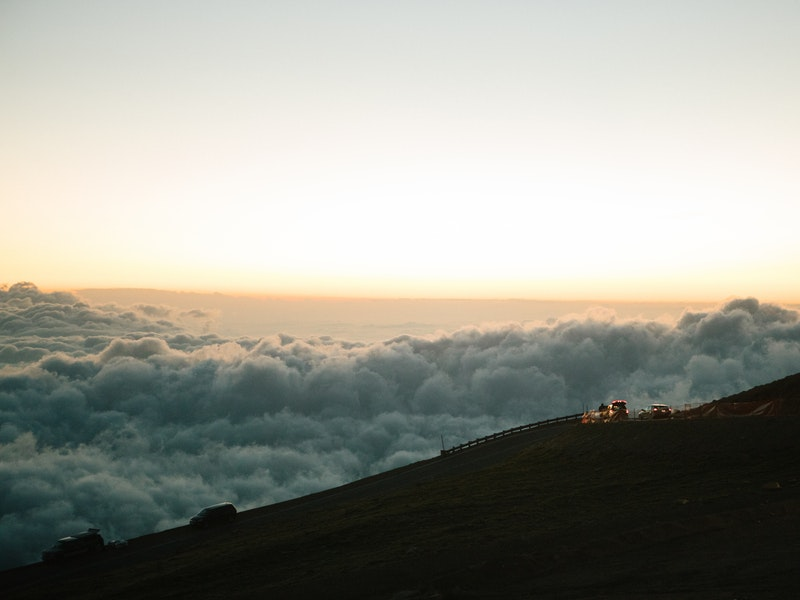
\includegraphics[scale=0.3]{../labwork/data/cloud.jpeg}
\caption{Original input image}
\end{figure}
\begin{figure}[h]
\center
\includegraphics[scale=0.3]{../labwork/build/labwork3-gpu-out.jpg}
\caption{Output image}
\end{figure}


\end{document}
